\subsection{SYN segment와 SYNACK segment의 역할}
    \subsubsection*{Terminology : Protocol Data Unit}
    프로토콜 데이터 단위\footnote{Protocol Data Unit}는 OSI 7 layer 구조로 표현할 수 있는 데이터통신에서
    상위 계층에서 전달한 데이터에 붙이는 제어정보를의미한다. 
    \vspace{-2mm}  
    \begin{wrapfigure}{l}{0.45\textwidth} \vspace{-20pt}
    \begin{center}
    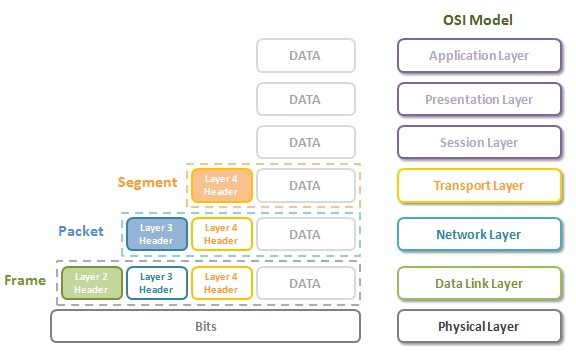
\includegraphics[width=0.45\textwidth]{image/week01/1-2-1.png}    
    \end{center}
    \vspace{-20pt}
    \caption{\small OSI 7 Layer}
    \vspace{-10pt}
    \end{wrapfigure}
    물리적으로 Bits로 표현되는 데이터에는 figure 에서 확인할 수 있는것과 같이 전송하고자 하는 데이터에
    각 Layer별로 기능을 수행하는 기능의 제어정보를 각각의 terminology를 사용해 표현되는 header에 
    추가해 줌으로서, Layer에 있는 Protocol이 기능을 수행할 수 있게 해준다.
    앞서 우리는 TCP의 기능을 확인해 보기 위해서 Network Layer의 제어정보인 Packet에 해당하는 TCP Header를 리뷰해 보았다.

    SYN segment 와 SYNACK segment는 Transport Layer에서 TCP의 제어정보를 담은 segment이고, TCP header의 flag field
    에서 확인한 SYN 과 ACK field와 연관이 있는 unit이다. 
    
    다루게될 UDP와 다르게 TCP는 연결지향\footnote{Connection Oriented} 동작을 하는 protocol로서 연속적인 데이터 전송의
    신뢰성을 보장해주는 기능을 수행하기위해 해당 segment들을 필요로한다. TCP는 패킷 전송 방식을 사용하기 때문에 보내려고 하는 데이터를 여러 개의 패킷으로 쪼개서 보낸다.

    이때 쪼개진 Packet들을 TCP를 이용해 통신하는 각 종단들은 어떤 TCP 옵션들을 사용할 지, 패킷의 순서 번호 동기화와 같이 통신에 필요한 몇 가지 segment들을 주고받는데, SYN segment와 SYNACK segment가 해당되고 이러한 최초 연결시의 
    동기화 과정을 \textbf{3-way handsake}라고 한다.
    \subsubsection*{TCP Connection : 3-way handsake}
    TCP가 통신을 시작할 때 거치는 과정을 3 Way Handshake, 통신을 마칠 때 거치는 과정을 4 Way Handshake 라고 한다.
    \vspace{-4mm}  
    \begin{figure}[!h]\centering
		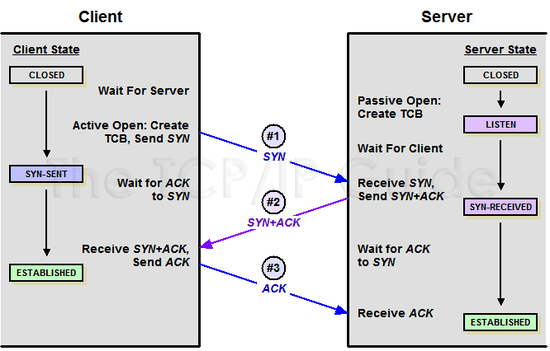
\includegraphics[width=.55\textwidth]{image/week01/1-2-2.png}
		\caption{\small 3-way handshake diagram}
		\vspace{-10pt}
    \end{figure}

    3way Handshake에서 3 Way라는 말 그대로 총 3번의 통신 과정을 거친다. 이 과정을 거치면서 통신을 하는 양 종단은 내가 누구랑 통신하고 있는지, 내가 받아야할 데이터의 시퀀스 번호가 몇 번인지와 같은 정보를 주고 받으면서 연결 상태를 생성하게 된다.
\clearpage
    \begin{figure}[h!]
    \centering
    \subfloat[The diagram of SYN sent using SYN segment]{
        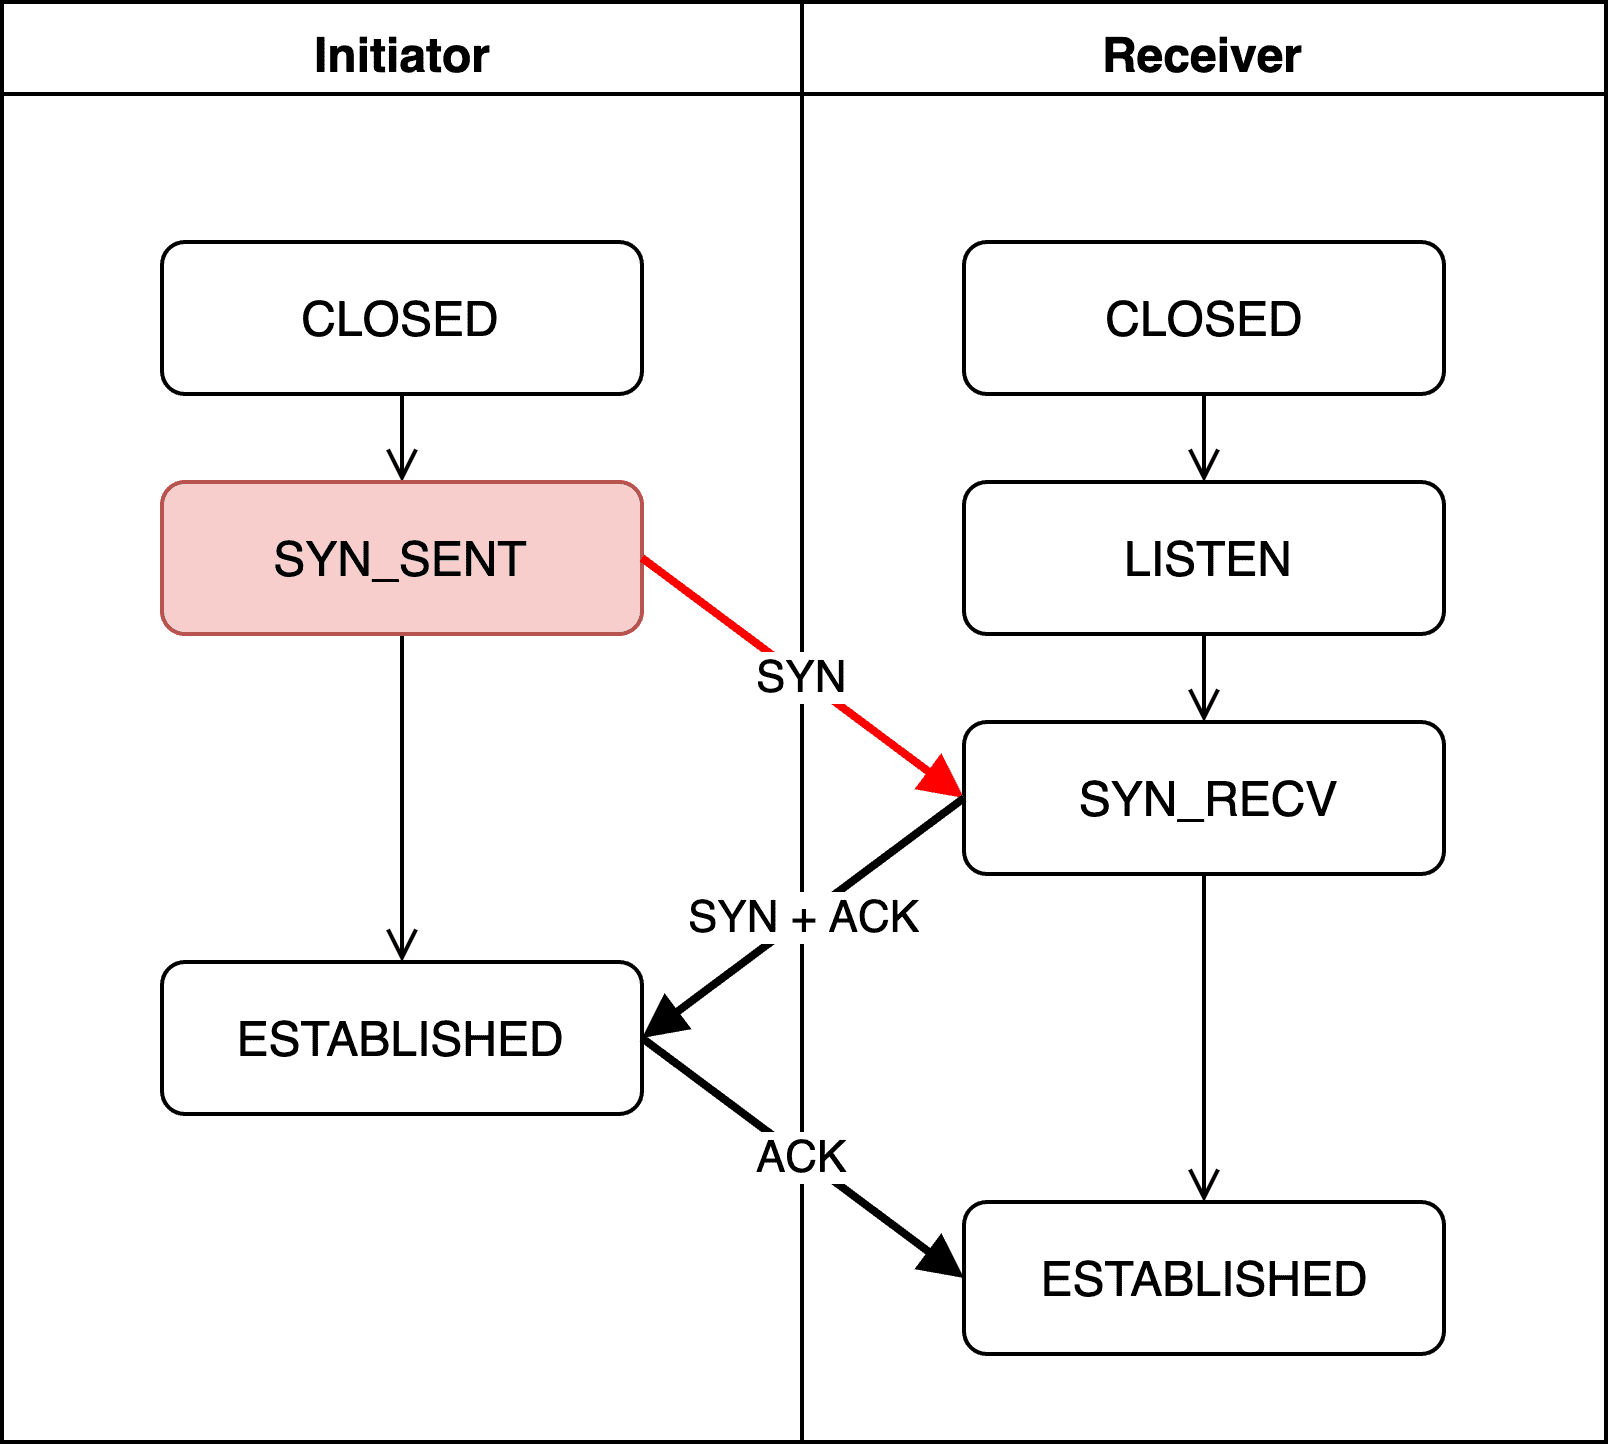
\includegraphics[width=0.45\textwidth] {image/week01/1-2-3.png}
    }\hspace{5mm}
    \subfloat[The diagram of SYN Received using SYNSCK segment]{
        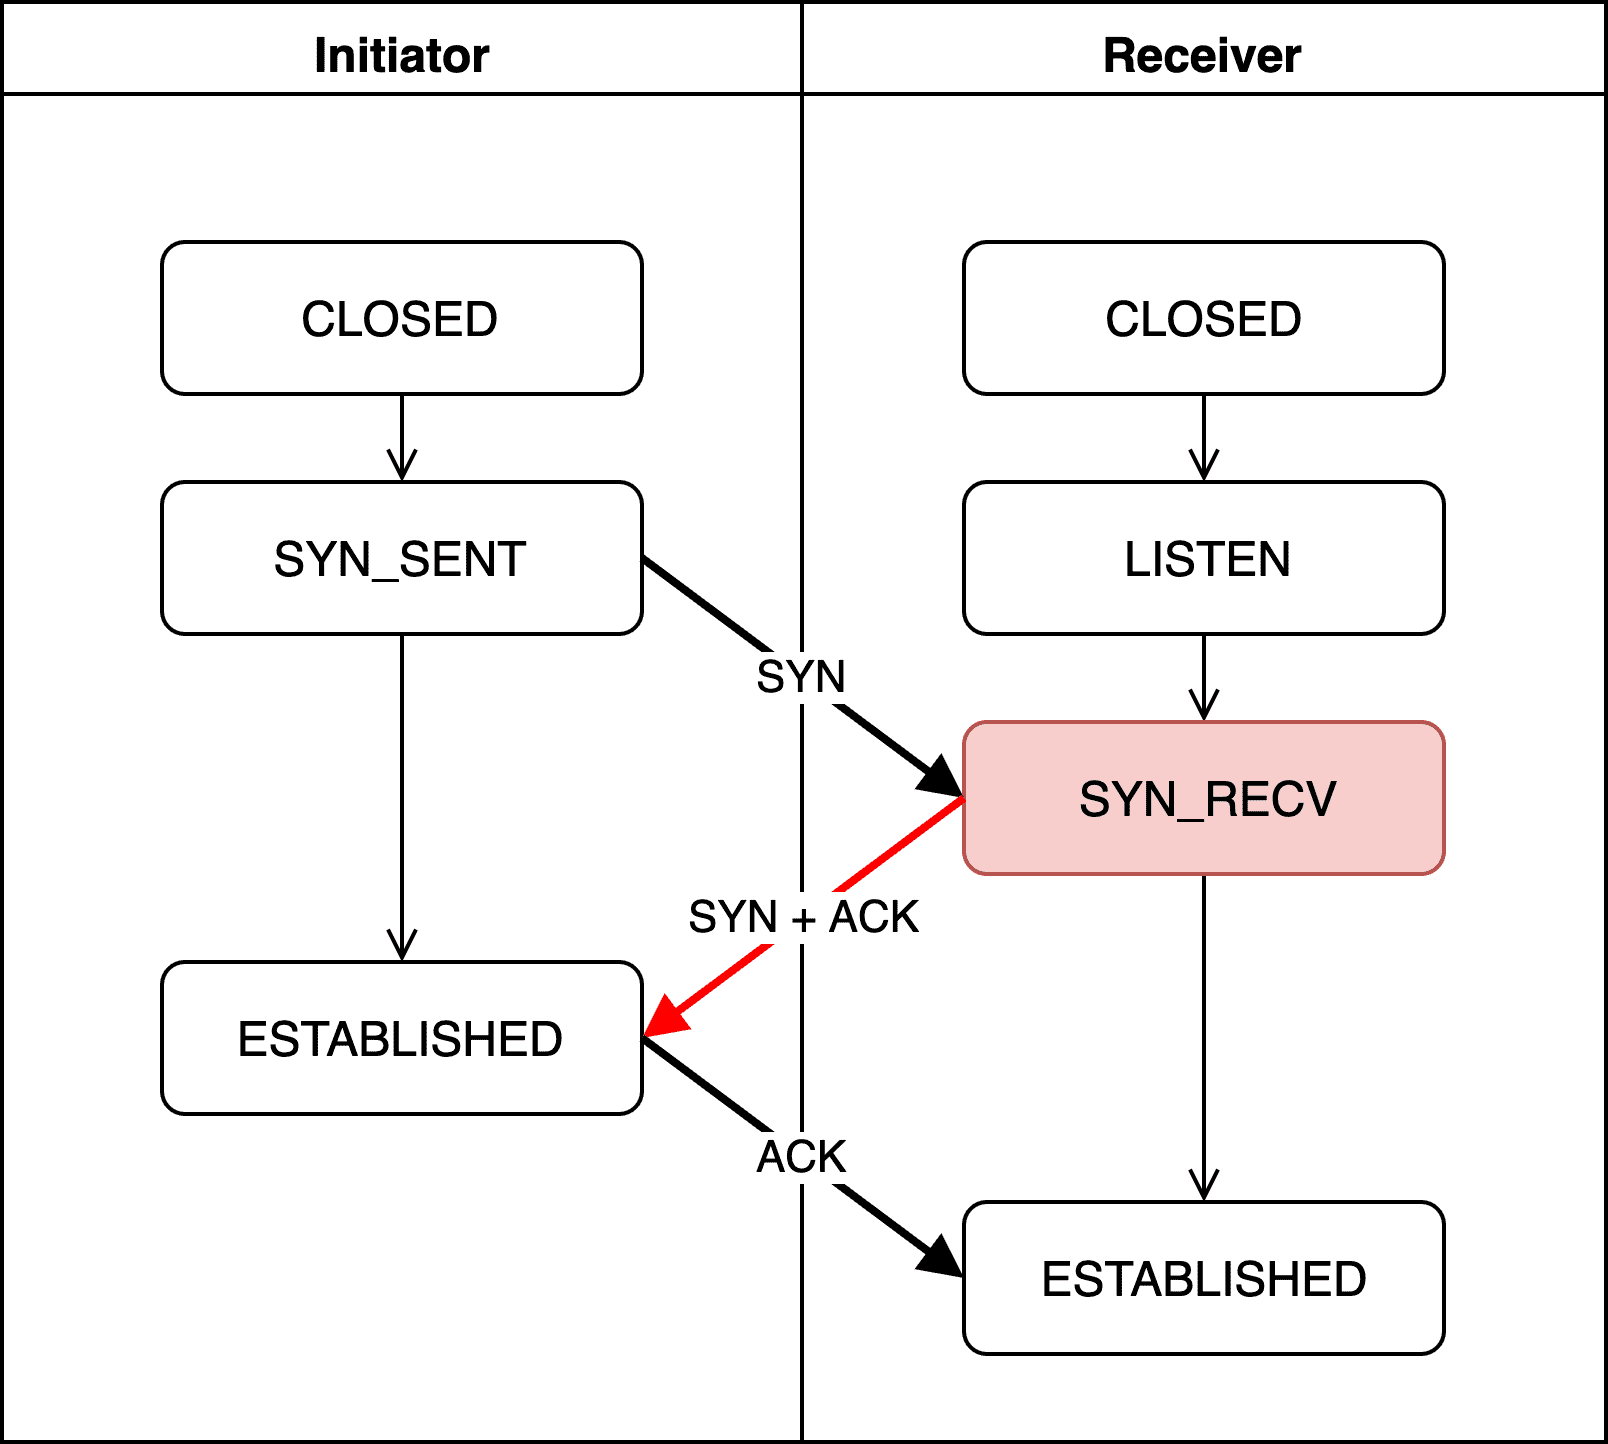
\includegraphics[width=0.45\textwidth] {image/week01/1-2-4.png}
    }\caption{3-way Handshake Process}
    \vspace{-2mm}
    \end{figure}
    \subsubsection*{SYN\_sent : SYN segment}
    요청자가 수신자에게 연결 요청을 하면서 랜덤한 숫자인 시퀀스 번호를 생성해서 SYN segment에 담아 보낸 상태이다. 이제 요청자와 수신자는 이 시퀀스 번호를 사용하여 계속 새로운 값을 만들고 서로 확인하며 연결 상태와 패킷의 순서를 확인하게 된다.
    \subsubsection*{SYN\_recv : SYNACK segment}
    SYN\_RECV는 요청자가 보낸 SYN 패킷을 수신자가 제대로 받은 상태를 의미한다.이후 수신자는 제대로 된 시퀀스 번호를 받았다는 확인의 의미인 `승인번호 Acknowledgement` 값을 만들어서 다시 요청자에게 돌려줘야한다. 이때 승인 번호는 처음 요청자가 보낸 시퀀스 번호 + 1이 된다.